\section{Zielgruppe, Problem, Eigenschaften, Alleinstellungsmerkmal}

\subsection{Zielgruppe}

Aufgrund der Coronapandemie wurden Konzepte wie Home-Office in vielen Industrien ausprobiert, in denen es so etwas zuvor wenig gab.
Mit diesen neuen Nutzern von dynamischen Arbeitsplatzkonzepten ist der potentielle Nutzerstamm für eine Anwendung zum dynamischen Zuweisen von Arbeitsplätzen stark gestiegen.
Maximal waren während der Pandemie in ein Umfrage der Hans-Böckler-Stiftung 27\% der Befragten im Home-Office.
Laut dem Ifo-Institut können ca 56\% aller Arbeitnehmer zumindest teilzeit im Home-Office Arbeiten. 
Das zeigt für wie viele Arbeitnehmer ein Dynamisches Arbeitsplatzkonzept wie unseres eine Möglichkeit wäre.

\begin{figure}[!h]
    \centering
    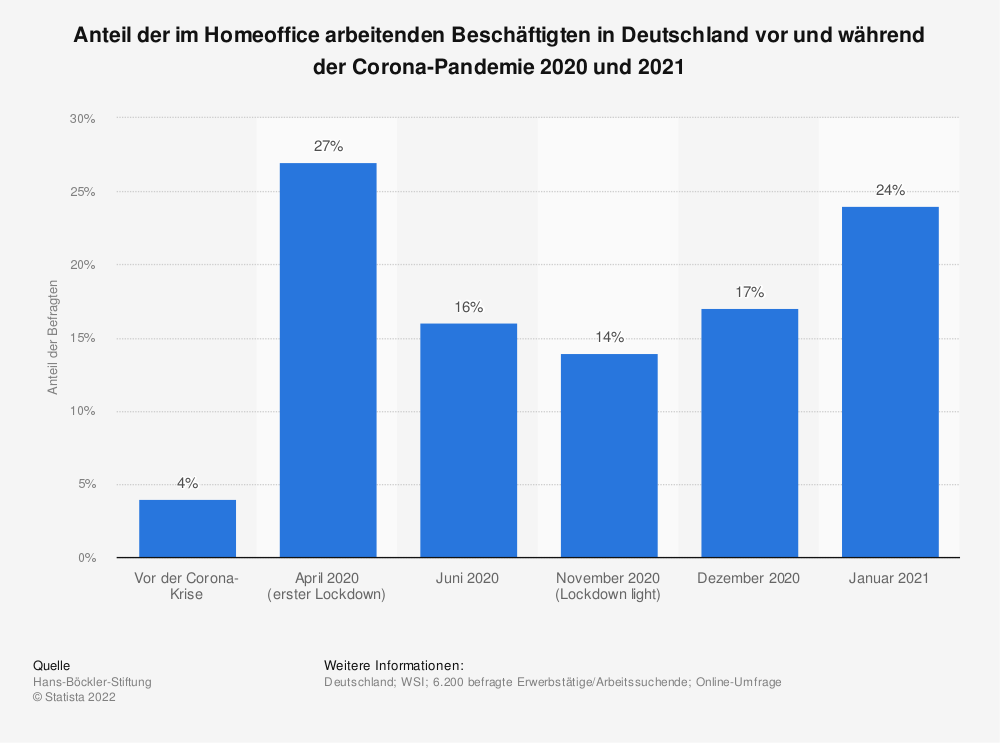
\includegraphics[width=0.8\textwidth]{statistik_homeoffice_corona.png}
    \caption{Home Office}
    \label{fig:HomeOffice}
\end{figure}

Dafür müssen aber auch Home-Office skeptische Arbeitgeber von den Vorteilen eines dynamischen Arbeitsplatzsystems, wie z.B. reduzierte Büro-Flächen und so geringere Miet- / Baukosten, überzeugt werden.
\pagebreak
\\
\textbf{Personas: }

\begin{figure}[!h]
    \centering
    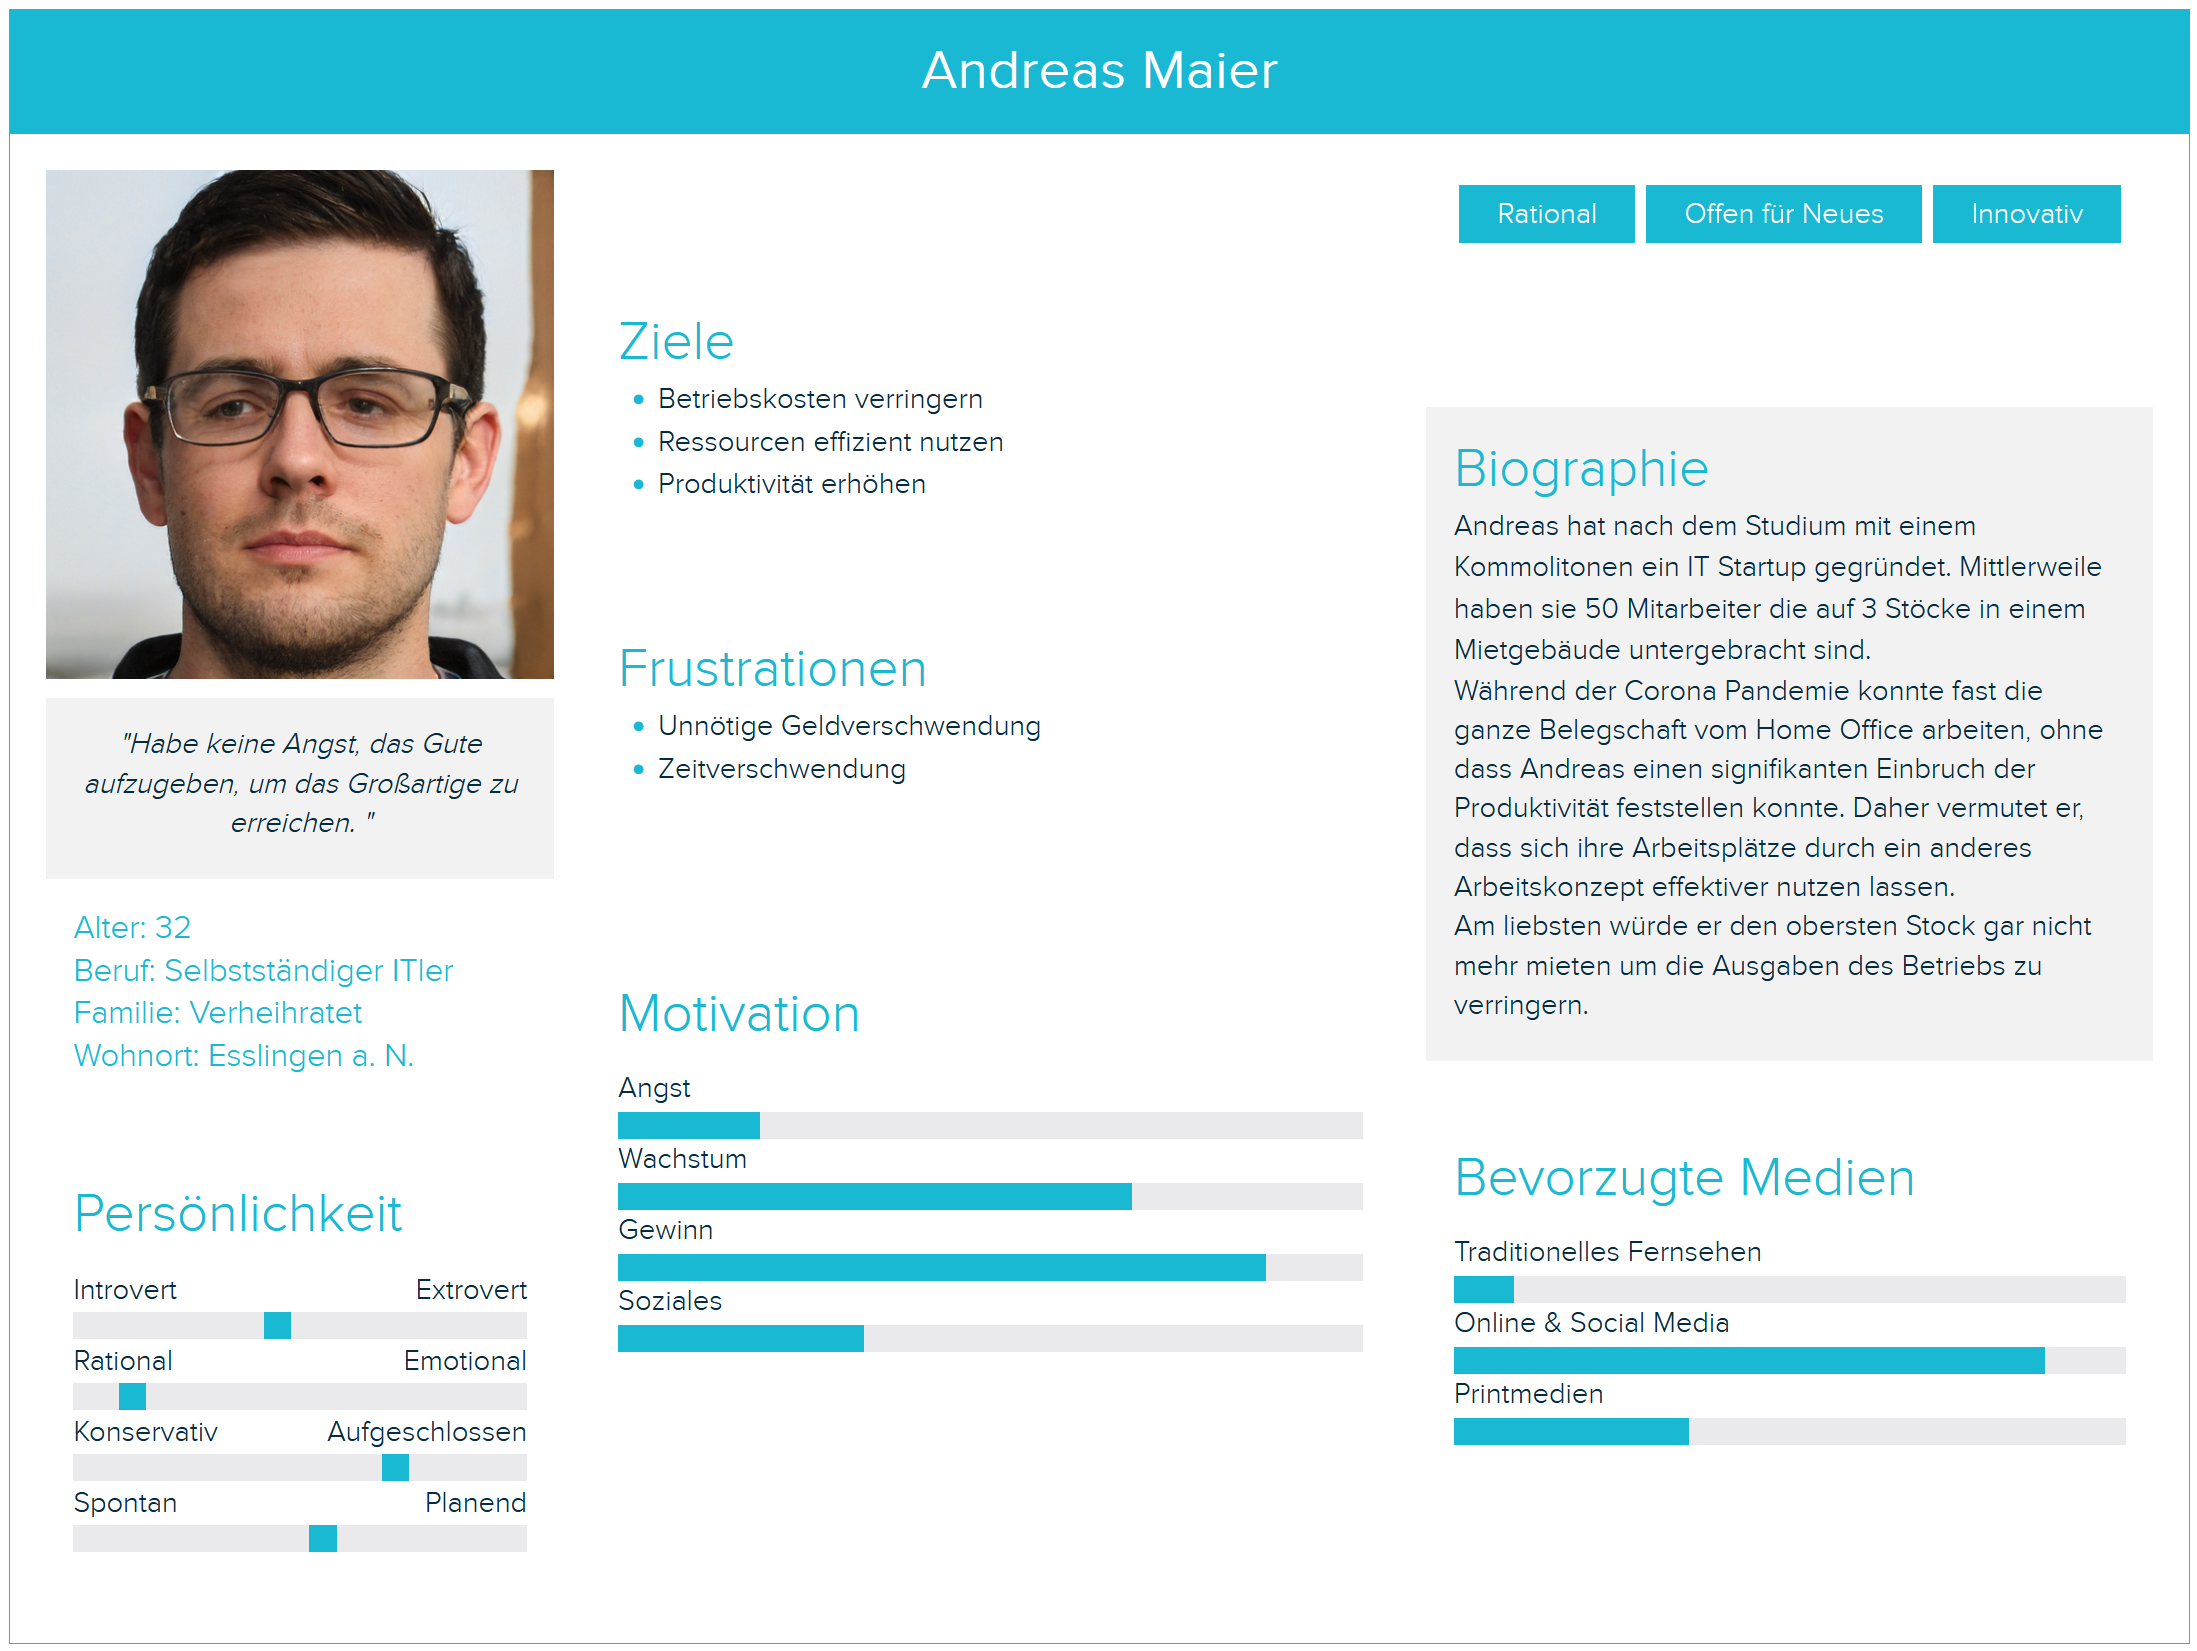
\includegraphics[width=1\textwidth]{Persona_Andreas_Maier.png}
    \caption{Persona Andreas Maier}
    \label{fig:PersonaAndreasMaier}
\end{figure}

Andreas repräsentiert den offensichtlichsten potentiellen Kunden.
Er erkennt selbst schon das Potential von nicht traditioneller Arbeitsplatznutzung und kommt schon von sich aus auf die Idee, nach den Erkenntnissen durch die Corona Zeit, die Arbeitsplatznutzung in seiner Firma umzustellen.\\
Er kann vermutlich mit rationalen Argumenten zur Kostenminderung, effizienten Zeitnutzung etc. von unserem Konzept überzeugt werden, hat aber auch hohe Ansprüche an Funktionalität und allgemeine Qualität der Anwendung.

\pagebreak

\begin{figure}[!h]
    \centering
    \includegraphics[width=1\textwidth]{Persona_Gerd_Ovelgönne.png}
    \caption{Persona Gerd Ovelgönne}
    \label{fig:PersonaGerdOvelgönne}
\end{figure}

Gerd ist Repräsentant einer konservativen Nutzergruppe, die noch nicht voll vom Konzept dynamischer Arbeitsplatzbelegung überzeugt sind, aber genug Motivationen haben, um potentiell von den Vorteilen überzeugt zu werden.
\\
Gerd ist schon sehr lange in seinem Beruf.
Er weiß genau was wie zu laufen hat und macht daher nur ungern Veränderungen.
\\
Durch die Vorgabe seiner Firma hat er jedoch eine externe Motivation, um das Arbeitskonzept seiner Abteilung zumindest ein wenig umzustellen.
Da Gerd zufriedene Mitarbeiter als Ziel hat, wäre das noch eine Motivation auf Umstellung, die wir in Werbung ansprechen könnten.
Den Mitarbeitern mehr Flexibilität zu bieten, sowohl in der reinen Wahl wo in der Abteilung sie sitzen als auch in der Entscheidung ob sie eine Arbeit von Zuhause erledigen können, kann sich positiv auf die Zufriedenheit der Mitarbeiter auswirken.
Vor allem wenn flexibleres Arbeiten durch die Vorgabe der Geschäftsführung in anderen Abteilungen möglich wird, sollten den eigenen Mitarbeitern auch ähnliche Möglichkeiten geboten werden um Frustration zu verhindern.
\\
Ihm sollten, da ihm Home-Office nicht so gefällt, auch Vorteile einer flexiblen Arbeitsplatznutzung ohne Home-Office gezeigt werden, wie bspw. die Einrichtung von Ruhearbeitszonen oder die Wahl der Arbeitsplätz entsprechend der Arbeit die an einem Tag stattfindet.


\subsection{Problem}
Während der Pandemiezeit wird verstärkt von Zuhause aus gearbeitet, dadurch schwankt die Anzahl der Arbeiter im Büro stark und die interdisziplinären Kollegen habe keinen Überblick mehr darüber, wer im Büro ist und wer nicht.
Zumal grundsätzlich nicht jeder in das Home-Office kann bzw. will, dies kann diverse Gründe, wie z. B. fehlende Räumlichkeiten oder die geschwächte Konzentrationsfähigkeit in den eigenen vier Wänden sein.
Agile Arbeitsplätze haben den Vorteil, dass der Arbeitsplatz je nach momentanem empfinden gewählt werden kann z. B. im sogenannten Ruhebereich, Bereiche die näher an Heizkörpern sind oder hellere Arbeitsplätze an Fenstern.
Projektspezifisch kann es vorteilhaft sein neben einem bestimmten Kollegen zu arbeiten, um den Austausch produktiver zu gestalten.
Diese Bereiche können frei benutzt werden, sofern diese nicht durch eine andere Kollegin oder einen anderen Kollegen belegt sind.
Derzeit ist es gängig, dass die Bereiche nach dem Prinzip “first come first serve“ besetzt werden. 

\paragraph{} Wenn man am Morgen an einem Arbeitsplatz sitzt, dann aber im Laufe des Tages für einen längeren Zeitraum diesen verlassen muss, wird diese Ressource unnötig blockiert.
Raumbelüftungssysteme, Heizungen und Klimaanlagen für Räume bzw. Gebäude werden nicht nach der Personenauslastung betrieben, in Hinblick auf die steigenden Energiekosten, ist dies weder ökonomisch noch nachhaltig.
Immungeschwächte Personen die ihre Tätigkeit nur vor Ort im Büro erledigen können, haben pandemiebedingt nicht die Möglichkeit Arbeitsplätze zu Buchen, die weiter weg von den restlichen Arbeitsplätzen bzw. Kollegen sind. 
Der Arbeitgeber, der nur eine bestimmte X Arbeitsplätzen hat, kann nicht mehr als X Arbeiter in dem Bürokomplex beschäftigen. 
Desweitern gibt es derzeit keine einfache Möglichkeit die Büro Belegschaft, über einen längeren Zeitraum zu analysieren. 
Diese Analyse kann unter anderem zur dauerhaften Arbeitsplatz Reduktion, bei gleicher Mitarbeiterzahl führen.

\paragraph{} Unsere Anwendung ermöglicht es, die oben angesprochenen Fälle zu Gunsten des Arbeitgebers und -nehmers zu lösen.
Die Raumplanung ermöglichet eine Buchung in 15 min Rastern auch Dauerbuchungen über mehrere Monate sind möglich.
Nicht nur Arbeitsplätze in einem Raum, sondern bestimmte Räume in bestimmten Gebäuden können gebucht werden.
Auch ist eine Chatfunktion zwischen Teamleitern und Mitarbeitern bzw. zwischen Mitarbeitern möglich.
Dies hat den Vorteil das Buchungen bei Sonderfällen unter Mitarbeitern einfach getauscht werden können.
Eine Synchronisation mit dem Outlookkalender wäre auch denkbar.

\subsection{Eigenschaften}
Die Web-Applikation DeskPlanner wird mindestens folgende Eigenschaften \\nachweisen können:

\begin{itemize}
    \item Open Source (Lizenzfrei) als kostenfreie Möglichkeit für vor allem kleine Unternehmen
    \item Simple Möglichkeiten, um Komplexität zu vermeiden, aber so viele Mög-lichkeiten der Raumplanung beizubehalten
    \item Three-Tier Architecture ähnliche Anwendungsweise der Raumplanung im Sinne von Gebäude > Stockwerk > Raum 
\end{itemize}

\paragraph{} Des Weiteren sind kleine Eigenschaften wie Einhaltung der 7 Usability Prinzipien vorgesehen, um so die Bedienung des Kunden so einfach wie möglich zu halten. 
Beispiele hierfür sind Hilfstexte, welche die verschiedenen Buttons erklären sollen oder selbsterklärende Icons der jeweiligen Buttons. 
Außerdem soll der Nutzer nicht mit Information beschüttet werden, sondern eine auf seinen Nutzungskontext angepasste Benutzeroberfläche sorgen für Aufgabenangemessenheit. 
Durch die individuelle Raumgestaltung erhält der Nutzer ein steuerbares Softwaresystem, welches genau das machen wird, was der Nutzer auch erwartet.

\subsection{Alleinstellungsmerkmal}
Als herausragendes Leistungsmerkmal des DeskPlanners bezeichnet man die effiziente Arbeitsplatznutzung. 
In der heutigen Branche, vor allem durch Corona bestätigt, gilt es, die Kosten immer weiter zu reduzieren. 
Durch die Raumbuchungsmöglichkeiten, kann ein Unternehmen die Arbeitsplätze minimieren, Home Office Mitarbeiter perfekt einplanen und dadurch Kosten der Technik und Größe des Raumes einsparen für andere Investitionen. 
Als Open Source Web-Applikation kann ein Unternehmen sogar lizenzfrei den Arbeitsplatz kosteneffizienter nutzen.
Genau hier soll der DeskPlanner vor allem kleineren Unternehmen unterstützen, um auch in Zeiten der Pandemie nicht insolvent zu gehen.
